% =====================================================================
% Appendix G: translation-unit pilot (one-column appendix).
% Ko<->En numbers (Blocks A, B; Figs. A8, A9) are measured and come from the
% archived score and analysis files of the pilot. Not cited on purpose (raw
% outputs not archived): oracle-LAAL ranges, collapse-free re-scores and
% duplicate re-emission counts. Block C (En<->De on TAXI) is planned.
% Do not claim significance, transfer to speech input, trained models or TAXI,
% that SEM_END beats the utterance end, or that the BLEU loss is paraphrase.
% =====================================================================
\section{Translation-Unit Pilot}\label{app:units}

This appendix reports a text-level pilot that motivates the translation commit units of \model (\cref{sec:model}). Its conditions differ from those of the benchmark: it simulates simultaneous translation over gold transcripts with gold word end times; it uses single-speaker Korean and English utterances from monolingual ASR corpora (150 per direction for quality, 300 per language for alignment statistics), not dialogues and not \pair{En}{De}; Qwen3.8-27B is the incremental translator; the references are offline translations by EXAONE-4.0-32B (silver references); and latency is computation-unaware LAAL on the gold word times. The pilot compares commit units under these conditions only and does not predict results for speech input, for trained models or on \taxi.

\paragraph{Commit policies.}
Let $u_{1:n}$ be the gold transcript of an utterance, $e_i$ the end time of word $u_i$, and $v_{1:J}$ the full offline translation by a teacher LLM. A policy commits translation text after it has read $b$ source words, and committed text is never revised, unlike in re-translation \citep{arivazhagan2020retranslation}. We compare four policies.
(i)~\emph{Utterance end} commits once, after $u_n$, which amounts to offline translation of the utterance.
(ii)~\emph{SEM\_END} commits at sentence-level semantic-completion boundaries: the positions at which an existing LLM-based labeller, which sees only the source transcript, judges the transcript so far semantically complete, i.e., later words will not change its meaning (in practice mostly the sentence-final punctuation of the transcript); the utterance end is added. These boundaries do not depend on the target language.
(iii)~\emph{Alignment-only meaning units (MU).} Contextual alignment \citep{labiausse2025highfidelity} assigns each target word $v_j$ to the source position $\alpha_j=\arg\max_{1\le i\le n}\,[L_j(i)-L_j(i-1)]$, where $L_j(i)$ is the summed log-probability of the tokens of $v_j$ when $v_{1:J}$ is force-decoded from $u_{1:i}$; ties go to the earliest $i$. A position $i$ is a \emph{valid cut} if the target words aligned at or before $i$ form a prefix $v_{1:k}$, so that, relative to the teacher's translation, the output up to that point need not change later. An \emph{MU boundary} is a valid cut that covers more target words than the previous valid cut; $n$ is always a valid cut and an MU boundary. This approximates, with alignment instead of generation, the translation-prefix consistency that defines meaning units (``meaningful units'' in \citealp{zhang2020learning}): minimal source segments whose translation is a prefix of the full translation. The policy commits at every MU boundary.
(iv)~\emph{Verified meaning units (MU2)} commit at a subset of the valid cuts. A candidate is a valid cut $b<n$ that covers more target words than the last commit $b'$ and lies at least a minimum unit after it: 2 Korean eojeol (space-delimited words) or 3 English words, and $e_b-e_{b'}\ge1.0$\,s. At a candidate, the translator receives the source heard so far and the committed translation in its prompt, rather than as a forced prefix, and writes only the new text. A language guard regenerates once and then rejects output in the wrong script: Han or Kana characters, Hangul in English output, or less than 30\% Hangul in Korean output. A generation check, in the spirit of \citet{zhang2020learning}, accepts the new text only if its sentence-level chrF \citep{popovic2015chrf} against the newly covered span $v_{k'+1:k}$ of the teacher's translation is at least $\theta=50$, where $k'$ is the coverage at the last commit. The rest of the utterance is translated at its end.

\paragraph{Setup.}
We sample 300 utterances per source language with word end times from monolingual Korean and English ASR corpora, plus a second, independent sample of the same size to check sample dependence; the source text is the gold transcript, and the SEM\_END positions are the labeller's output for it. The labeller has LLM judges rate candidate positions, proposed by an LLM or by rules (e.g., at sentence-final punctuation), and keeps a candidate if its ratings pass thresholds set per candidate type so that precision against LLM-annotated reference labels is at least 0.90 on a development split. Alignments come from Qwen3.8-27B on both samples and from EXAONE-4.0-32B on the first. The quality runs use 150 utterances per direction from the first sample (mean length 11.09\,s for Korean and 15.05\,s for English sources), with Qwen3.8-27B as translator and as the MU2 teacher. The references are EXAONE-4.0-32B offline translations of the full gold transcripts, from another model family than the translator; no human references exist for these utterances. Teachers and reference translator receive \textit{``Translate the following $\langle$src$\rangle$ speech transcript into natural $\langle$tgt$\rangle$. Output only the $\langle$tgt$\rangle$ translation, nothing else.''}, followed by the transcript.
\draftnote{name the source corpora, the sampling arguments and the origin of the word times; the Korean transcripts seem to be filtered ASR output, so verify before calling them gold}

Block A of \cref{tab:units} runs the utterance end, SEM\_END and MU2 with one incremental prompt and the language guard; only MU2 adds the minimum unit and the generation check. The prompt reads
\begin{quote}\small\itshape
You are a simultaneous interpreter translating $\langle$src$\rangle$ speech into $\langle$tgt$\rangle$.\\
Source heard so far: $\langle$source prefix$\rangle$\\
Translation already given (cannot be changed): $\langle$committed text, or ``(none)''$\rangle$\\
Translate only the part of the source that the translation already given does not cover yet, continuing it naturally in $\langle$tgt$\rangle$. [The speaker is still talking: translate only what has been said so far and do not guess the rest.] Output only the new $\langle$tgt$\rangle$ text, nothing else. If nothing new can be translated yet, output nothing.
\end{quote}
where the bracketed sentence appears only before the end of the utterance, and a regeneration by the guard appends \textit{``Write the answer in $\langle$tgt$\rangle$ only.''} Block B runs the utterance end, SEM\_END and alignment-only MUs with the offline prompt, which before the end of the utterance also says \textit{``The transcript may be incomplete because the speaker is still talking: translate only what has been said so far, do not guess or complete the rest.''}; the committed text is forced as the beginning of the answer, and the continuation is committed. Block B has no language guard, and its latency was not reported. In both blocks, the utterance-end translation may use up to 160 tokens and every other step at most $\min(160,\,2\ell+8)$, where $\ell$ is the token length of the utterance-end translation, and an $m$-gram ($m\le3$) repeated three or more times in a row is cut.

We report corpus BLEU \citep{papineni2002bleu} and chrF with sacreBLEU \citep{post2018call}, with the BLEU tokenizer \texttt{intl} for Korean and \texttt{13a} for English output; chrF is primary for Korean output. An output \emph{collapses} if it is empty, is in the wrong script as defined for the guard, or contains an $m$-gram ($m\le3$) repeated three or more times in a row. Latency ignores LLM computation and ASR delay. Output word $j$ gets the commit time $d_j=e_b$ of the step that wrote it, and per utterance
\[
  \mathrm{LAAL}=\frac{1}{\tau}\sum_{j=1}^{\tau}\Bigl(d_j-(j-1)\,\frac{e_n}{|Y|}\Bigr),
\]
where $|Y|$ is the output length in words and $\tau$ the first $j$ with $d_j=e_n$ (or $|Y|$ if there is none). This is the length-adaptive form \citep{papi2022overgeneration} of Average Lagging \citep{ma2019stacl}, except that $|Y|$ replaces $\max(|Y|,|Y^*|)$ with the reference length $|Y^*|$; the two agree whenever the output is at least as long as the reference. \emph{First commit} is $d_1$. Both are averaged over utterances, so the LAAL of the utterance end equals the mean utterance length.
\draftnote{recompute LAAL with $\max(|Y|,|Y^*|)$ when the raw outputs are re-exported}
For the alignment statistics, a source word $u_i$ waits $e_{b(i)}-e_i$ until the first boundary $b(i)\ge i$ of a policy.

% =====================================================================
% Table A10 (tab:units): text-level commit-unit pilot. Included from App. G.
% Blocks A and B (Ko<->En) are measured: values copied from the archived score
% files of the pilot (prompt-based run = Block A; forced-prefix run = Block B).
% Block B: no latency was reported, nor collapse counts for its utterance-end
% and SEM_END rows ("--").
% Block C (En<->De on TAXI gold transcripts) is planned: every cell is \tbd.
% =====================================================================
\begin{table}[t]
  \caption{Text-level commit-unit pilot (\cref{app:units}). Blocks A and B: \pair{Ko}{En}, 150 single-speaker utterances per direction, fixed transcripts (Korean: ASR output kept when two recognisers agree) with forced-aligned word end times, Qwen3.8-27B as translator, silver references (offline EXAONE-4.0-32B translations) and computation-unaware LAAL. The two blocks use different prompts, so rows are compared only within a block. Block C (planned): \pair{En}{De} \taxi turns with gold transcripts and forced-aligned word times, scored by \scorer against the human references; its left group is \deen, its right group \ende, and its LAAL is \laal on the ideal clock. LAAL and First (commit time of the first output word) in seconds. Coll.: collapsed outputs (empty, wrong script or a repetition loop), out of 150 in Blocks A and B. Candidates accepted: MU2 candidates that pass the language guard and the chrF check. --: not reported; blank: pending.}
  \label{tab:units}
  \centering
  \small
  \setlength{\tabcolsep}{4.5pt}
  \begin{tabular}{@{}lcccccccccc@{}}
    \toprule
    & \multicolumn{5}{c}{\koen (C: \deen)} & \multicolumn{5}{c}{\enko (C: \ende)} \\
    \cmidrule(lr){2-6}\cmidrule(l){7-11}
    Block\,/\,commit policy & BLEU & chrF & LAAL & First & Coll. & BLEU & chrF & LAAL & First & Coll. \\
    \midrule
    \multicolumn{11}{@{}l}{\textit{A: prompt-based commits}} \\
    Utterance end             & 35.2 & 61.3 & 11.09 & 11.09 & 0 & 23.4 & 44.2 & 15.05 & 15.05 & 1 \\
    SEM\_END                  & 35.3 & 61.1 &  7.49 &  8.23 & 0 & 22.4 & 43.7 &  8.63 &  9.74 & 0 \\
    Verified MU (MU2)         & 31.1 & 60.2 &  5.19 &  7.03 & 0 & 19.9 & 42.0 &  7.33 &  8.25 & 1 \\
    \quad candidates accepted & \multicolumn{5}{c}{197/368 (54\%)} & \multicolumn{5}{c}{185/873 (21\%)} \\
    \midrule
    \multicolumn{11}{@{}l}{\textit{B: forced-prefix continuation (latency not reported)}} \\
    Utterance end             & 32.9 & 58.4 & -- & -- & -- & 21.2 & 42.3 & -- & -- & -- \\
    SEM\_END                  & 34.4 & 59.2 & -- & -- & -- & 19.2 & 40.8 & -- & -- & -- \\
    Alignment-only MU         & 28.1 & 54.2 & -- & -- & 5  & 12.9 & 33.1 & -- & -- & 31 \\
    \midrule
    \multicolumn{11}{@{}l}{\textit{C: \pair{En}{De} \taxi turns, human references (planned)}} \\
    Turn end                  & \tbd & \tbd & \tbd & \tbd & \tbd & \tbd & \tbd & \tbd & \tbd & \tbd \\
    Verified MU (MU2)         & \tbd & \tbd & \tbd & \tbd & \tbd & \tbd & \tbd & \tbd & \tbd & \tbd \\
    \quad candidates accepted & \multicolumn{5}{c}{\tbd} & \multicolumn{5}{c}{\tbd} \\
    \bottomrule
  \end{tabular}
\end{table}


\paragraph{Verified meaning units halve the lag.}
In Block A (\cref{tab:units,fig:units}), MU2 roughly halves LAAL relative to the utterance end, from 11.09 to 5.19\,s (\koen) and from 15.05 to 7.33\,s (\enko), stays below SEM\_END (7.49 and 8.63\,s), and makes its first commit earlier (7.03 against 11.09\,s and 8.25 against 15.05\,s). chrF falls from 61.3 to 60.2 and from 44.2 to 42.0; BLEU falls more, from 35.2 to 31.1 and from 23.4 to 19.9. Whether this reflects paraphrase or errors is untested, since the references are silver and no human judged the outputs. SEM\_END scores close to the utterance end, but its output is identical to the utterance-end output in 96/150 (\koen) and 83/150 (\enko) utterances.

\begin{figure}[t]
  \centering
  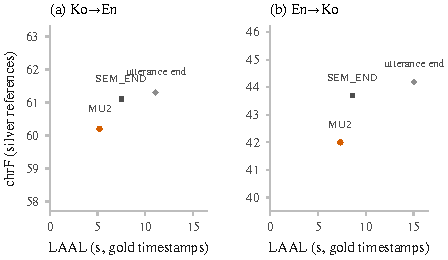
\includegraphics{figures/figA8_unit_quality_latency.pdf}
  \caption{Commit-unit pilot, Block A of \cref{tab:units}: chrF against computation-unaware LAAL for (a)~\koen and (b)~\enko (text level; 150 utterances per direction; gold transcripts and word times; silver references). Verified meaning units (MU2) roughly halve LAAL relative to committing at the utterance end, at a small chrF cost; SEM\_END lies in between on both axes. The LAAL of the utterance end equals the mean utterance length.}
  \label{fig:units}
\end{figure}

\paragraph{SEM\_END is sentence-level.}
Across the three alignment runs, an utterance contains 1.16--1.44 SEM\_END units against 3.09--3.45 MUs for Korean sources, and 1.75--1.88 against 5.52--5.73 for English sources. A SEM\_END unit spans 11.83--12.82 eojeol against 5.70--6.73 for an MU in Korean, and 24.68--26.15 against 9.22--9.93 words in English (\cref{fig:unit-gran}). Of all SEM\_END positions, 42.3--85.9\% coincide with the utterance end, which is a valid cut by definition; counting these, 79.6--92.2\% are valid cuts. Yet SEM\_END positions cover only 2.0--8.1\% of the MU boundaries inside utterances, and a source word waits 3.75--4.05\,s (Korean) and 5.20--5.73\,s (English) for the next SEM\_END boundary, against 2.59--3.25\,s and 3.22--3.38\,s for the next MU boundary. Semantic completion of the source therefore marks few of the points at which a translation could already be committed.
\draftnote{also report the valid-cut share of the SEM\_END positions inside utterances}

\begin{figure}[t]
  \centering
  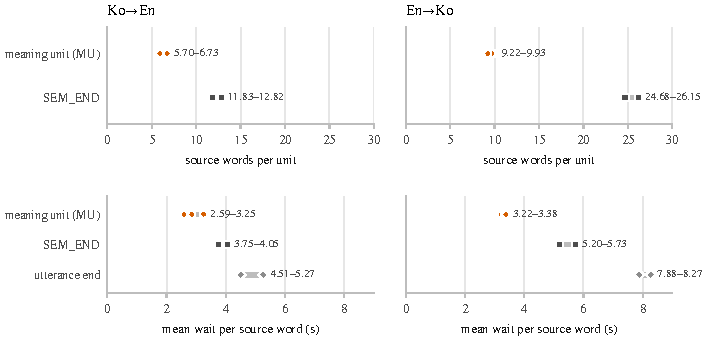
\includegraphics{figures/figA9_unit_granularity.pdf}
  \caption{Unit granularity on 300 utterances per source language: source words per unit (Korean: eojeol) and mean wait of a source word until the next commit boundary, for alignment-only meaning units (MU), SEM\_END and the utterance end. Dots are three alignment runs (Qwen3.8-27B and EXAONE-4.0-32B on one sample; Qwen3.8-27B on a second sample); bars span the minimum to the maximum. SEM\_END and utterance-end values depend on the sample but not on the teacher.}
  \label{fig:unit-gran}
\end{figure}

\paragraph{Unverified units collapse, and acceptance depends on the direction.}
Block B commits without verification: alignment-only MUs continued from a forced prefix collapse in 5/150 \koen and 31/150 \enko outputs, through text in another script (including copied source), loops or empty output, and their chrF drops to 54.2 and 33.1, against 58.4 and 42.3 for the utterance end of the same block. MU2 collapses in 0/150 and 1/150 utterances; the single \enko case is an utterance whose utterance-end output is empty as well. MU2 differs from Block B's MUs in its prompt, the guard, the minimum unit and the check at once, so the pilot does not separate their effects. The check accepts 197 of 368 candidates (54\%) for \koen but only 185 of 873 (21\%) for \enko; nearly all rejections fail the chrF threshold (171 and 685; the other three \enko rejections are one empty and two wrong-language outputs). This is consistent with Korean word order: a Korean translation places the verb last, so the translation of an English prefix rarely matches the span of the full translation aligned to it. With so few accepted candidates, \enko MU2 is only 1.3\,s faster than SEM\_END, and its output equals the utterance-end output in 52/150 utterances (32/150 for \koen).

\paragraph{Extension to \pair{En}{De}.}
Block C of \cref{tab:units} repeats the comparison on the main pair with human references: \taxi turns with gold transcripts and forced-aligned word times, Qwen3.8-27B as alignment teacher and translator, $\theta=50$, a German minimum unit set on held-out data, and trimming of committed text that is re-emitted at the turn end; \scorer scores the output against the TAXI references. Its MU2 row is the oracle-transcript streaming bound of \cref{tab:main}. TAXI turns are much shorter than the pilot utterances (mean source turn 3.086\,s in German and 4.624\,s in English; mean pilot utterance 11.09\,s in Korean and 15.05\,s in English), which bounds what commits inside a turn can gain.
\draftnote{planned; Block C has not been run}

\paragraph{Limitations.}
The references are silver translations by one LLM, with no human references, COMET or human judgement. The utterances are long, come from single-speaker monolingual corpora and are not dialogues. Transcripts and word times are gold, latency ignores computation and ASR delay, and LAAL is computed per utterance rather than as session-level \laal. There are no confidence intervals: with 150 utterances per direction, small differences, such as between SEM\_END and the utterance end, are not interpreted. The translator, the alignment teacher and the target of the generation check are the same model (Qwen3.8-27B), so the check may favour its own phrasing, and neither $\theta$ nor the minimum unit was tuned. Finally, MU2 sometimes re-emits committed text at the utterance end; the pilot does not trim it, which may inflate the \koen length ratio of MU2 (1.13, against 1.05 for the utterance end).
